%\section{Bounds on the number of types}\label{sec:types}
\subsection{Bounds on the number of types}%\label{sec:types}



We now come to the proof of \autoref{thm:vc-density}.
%
%In this section we prove \autoref{thm:vc-density} and \autoref{thm:vc-density-lower-bound}.
%	Recall that \autoref{thm:vc-density} provides upper bounds on the number of types in classes of graphs which are nowhere dense, 
%	and stronger bounds for classes which have bounded expansion. 
%	On the other hand, the complementary \autoref{thm:vc-density-lower-bound} shows that for subgraph-closed classes, in the absence of structural sparsity we cannot hope for such upper bounds.
%
%\subsection{Upper bounds for sparse classes}
%We first prove \autoref{thm:vc-density}, which we recall for convenience.
%
%%\vcupper*
%% \setcounter{aux}{\thetheorem}
%% \setcounter{theorem}{\thevcupper}
% \begin{theorem}\label{thm:vc-density-recall}
% Let $\CCC$ be a class of graphs and let $\phi(\tup x,\tup y)$ be a first order formula
% with free variables  partitioned  into object variables $\bar x$  and parameter variables $\bar y$. Let $\ell=|\bar x|$. Then:
% \begin{enumerate}
% \item If $\CCC$ is nowhere dense, then for every $\epsilon>0$
% there exists a constant~$c$ such that for every $G\in \CCC$ and every nonempty
% $A\subseteq V(G)$, we have $|S^\phi(G/A)|\leq c\cdot |A|^{\ell+\epsilon}.$
% \item If $\CCC$ has bounded expansion, then there exists a constant~$c$ such that for every $G\in \CCC$ and every nonempty $A\subseteq V(G)$, we have $|S^\phi(G/A)|\leq c\cdot |A|^\ell$.
% \end{enumerate}
% \end{theorem}
%% \setcounter{theorem}{\theaux}
%We remark that the theorem holds also for colored graphs, in the following sense.
%A class of graphs  whose vertices and edges are colored by a fixed finite number of colors is nowhere dense if the underlying class of graphs obtained by forgetting the colors is nowhere dense. 
%Then~\autoref{thm:vc-density} holds also for such classes of colored graphs, with the same proof. Namely, all graph theoretic notions
%are applied to the underlying colorless graphs, only the definition of types takes the colors into account. 
%The results of~\autoref{sec:gaifman} then need to be lifted to edge- and vertex-colored graphs, but this is straightforward.
%
%\medskip
%The proof of~\autoref{thm:vc-density} spans the remainder of this section.
In the proof, we will
will first enlarge the set $A$ to a set $B$, called
an \emph{$r$-closure of~$A$} (where $r$ is chosen depending on $\phi$), such 
that the connections of elements from $V(G)-B$ 
toward $B$ are well controlled. This approach
was first used in Drange et al.~\cite{drange2016kernelization} in the context of classes of bounded expansion, 
and then for nowhere dense classes in Eickmeyer et al.~\cite{eickmeyer2016neighborhood}. 
We start by recalling these notions.

Let $G$ be a graph and let $B\subseteq V(G)$ be a subset of vertices. For vertices $v\in B$ and $u\in V(G)$, a path $P$ leading from $u$ to $v$ is called {\em{$B$-avoiding}}
if all its vertices apart from~$v$ do not belong to~$B$. Note that if $u\in B$, then there is only one $B$-avoiding path leading from $u$, namely the one-vertex path where $u=v$.
For a positive integer $r$ and $u\in V(G)$, the {\em{$r$-projection}} of $u$ on $B$, denoted $M^G_r(u,B)$, is the set of all vertices $v\in B$ such that there is
a $B$-avoiding path of length at most $r$ leading from $u$ to $v$. Note that for $u\in B$, we have $M^G_r(u,B)=\{b\}$.
Equivalently, $M^G_r(u,B)$ is the unique inclusion-minimal
subset of $B$ which $r$-separates $u$ from $B$.
% (cf.~Fig.~\ref{fig:projection}).
%
%\begin{figure}[h!]
%	\centering
%		\includegraphics[scale=0.35,page=2]{pics}
%	\caption{The  $r$-projection of $u$ on $B$
%	(here $r=2$)
%	is the minimal set  $S\subset B$
%	which $r$-separates $ u$ from $B$.
%	}
%	\label{fig:projection}
%\end{figure}
%
%We will use the following results from~\cite{drange2016kernelization,eickmeyer2016neighborhood}.
We will use the following result from~\cite{eickmeyer2016neighborhood}.

%\begin{lemma}[\cite{drange2016kernelization}]\label{lem:closure-be}
%Let $\CCC$ be a class of bounded expansion. 
%Then for every $r\in \N$ there is a constant $c\in \N$ such that for
%every $G\in \CCC$ and $A\subseteq V(G)$ there exists a set $B$, called an {\em{$r$-closure}} of $A$, with the following properties:
%\begin{enumerate}%[(a)]
%  \item $A\subseteq B\subseteq V(G)$;
%  \item $|B|\leq c\cdot |A|$; and
%  \item $|M_r^G(u,B)|\leq c$ for each $u\in V(G)$.
%  \end{enumerate}
%  Moreover, for every set $X\subset V(G)$, it holds that
%  \begin{enumerate}%[(d)]
%  \item $|\setof{M_r^G(u,X)}{u\in V(G)}|\leq c\cdot |X|$.
%\end{enumerate}
%\end{lemma}

\begin{lemma}[\cite{eickmeyer2016neighborhood}]\label{lem:closure-nd}
Let $\CCC$ be a nowhere dense class. 
Then for every $r\in\N$ and $\delta>0$ there is a 
constant $c\in\N$ such that for every $G\in \CCC$ and $A\subseteq V(G)$ there exists a set 
$B$,  called an {\em{$r$-closure}} of $A$, 
with the following properties: 
\begin{enumerate}%[(a)]
  \item $A\subseteq B\subseteq V(G)$;
  \item $|B|\leq c\cdot |A|^{1+\delta}$; and
  \item $|M_r^G(u,B)|\leq c\cdot |A|^{\delta}$ for each $u\in V(G)$.
  \end{enumerate}
  Moreover, for every set $X\subset V(G)$, it holds that
  \begin{enumerate}  
  \item[4.] $|\setof{M_r^G(u,X)}{u\in V(G)}|\leq c\cdot |X|^{1+\delta}$.
\end{enumerate}
\end{lemma}

We note that in~\cite{drange2016kernelization,eickmeyer2016neighborhood} projections on $B$ are defined only for vertices outside of $B$. 
However, adding singleton projections for vertices of $B$ to the definition only adds $|B|$ possible projections of size $1$ each, so this does not influence the validity of the above results.


We proceed with the proof of \autoref{thm:vc-density}.
% To focus attention, we present the proof only for the nowhere dense case (first statement). The proof in the bounded expansion case (second statement)
% can be obtained by replacing all the parameters $\epsilon,\delta,\epsilon_1,\epsilon_2$ below by~$0$, and substituting the usage of Theorem~\ref{lem:closure-nd} with Theorem~\ref{lem:closure-be}.
%
 Let us fix: a nowhere dense class of graphs $\CCC$, a graph $G\in \CCC$, a vertex subset $A\subseteq V(G)$, a real $\epsilon>0$, and 
 a first order formula $\phi(\bar x,\bar y)$, where $\bar x$ is the distinguished $\ell$-tuple of object variables.
 Our goal is to show that $|S^\phi(G/A)|=\Oof(|A|^{\ell+\epsilon})$.
 	   
In the sequel, $d$ denotes a positive integer 
depending on ${\cal C},\ell,\phi$ only (and not on $G, A$ and $\epsilon$), and will be specified later. We may choose positive reals
$\delta,\epsilon_1$ such that 
	 $(\ell+\epsilon_1)(1+\delta) 
	 \le
	 \ell+\epsilon$ and $\epsilon_1>\delta(d+\ell)> \delta\ell$, for instance as follows: $\epsilon_1=\epsilon/2$ and $\delta=\frac{\epsilon}{4d+4\ell}$.
The constants hidden in the $\Oof(\cdot)$ notation below depend
 on $\epsilon,\delta,\epsilon_1,\cal C, \ell$ and $\phi$, but not on $G$ and $A$.   By \emph{tuples} below we refer to tuples of length $\ell$.

	Let $q$ be the quantifier rank of $\phi$ and let 
$p,r$ be the numbers obtained by applying Lemma~\ref{lem:types} to $q$ and $\ell$.
Let $B$ be an $r$-closure of $A$, given by Lemma~\ref{lem:closure-nd}.
  By Lemma~\ref{lem:closure-nd}, the total number of distinct $r$-projections onto $B$ 
  is at most $\Oof(|B|^{1+\delta})$, and each of these projections has size $\Oof(|B|^{\delta})$.
%
  	   Figure~\ref{fig:sketch} serves as  an illustration to the steps of the proof in the case $\ell=1$.
  	   \begin{figure*}[h!]
  	   	\centering
  	   		\includegraphics[width=\textwidth,page=4]{pics}
          %code
          % \noindent\textbf{Claim 1}. $X$ -- set of nodes\\
%           with distinct $\varphi$-types over $B$.\\
%           Then $|X|={\cal O}(|B|^{1+\varepsilon_1})$.
%
%           \medskip
%           \noindent\textbf{Claim 2}. $Y\subseteq X$ -- set of nodes\\
%           with the same projection $C$.\\
%           Then $|Y|={\cal O}(|B|^{\varepsilon_2})$.
%
%           \medskip
%           \noindent\textbf{Claim 3}. $Z\subseteq Y$\\
%           mutually $2r$-separated by $S$.\\
%           Then $|Z|={\cal O}(|C|)$.
  			\caption{The proof of~\autoref{thm:vc-density} in case $\ell=1$. 
  The logical implications flow from right to left,
  but our description below proceeds in the other direction.
  			}
  	   	\label{fig:sketch}
  	   \end{figure*}	
	
	\setcounter{claim}{0}
%	
The first step is to reduce the statement to the following claim.

\begin{claim}\label{claim2}
If $X$ is a set of tuples with pairwise different $\phi$-types over $B$, then $|X|=\Oof(|B|^{\ell+\epsilon_1})$.
\end{claim}	

Claim~\ref{claim2} implies that $|S^\phi(G/B)|=\Oof(|B|^{\ell+\epsilon_1})$, 
which is bounded by $\Oof(|A|^{(\ell+\epsilon_1)(1+\delta)})$ since $|B|=\Oof(|A|^{1+\delta})$. 

As $(\ell+\epsilon_1)(1+\delta)\le \ell+\epsilon$, this shows that $|S^\phi(G/B)|=\Oof(|A|^{\ell+\epsilon})$.
Since $A\subset B$, 
we have $|S^\phi(G/A)|\le |S^\phi(W/B)|$ so
 $|S^\phi(G/A)|=\Oof(|A|^{\ell+\epsilon})$, and we are done. Therefore, it remains to prove Claim~\ref{claim2}.

\medskip

For a tuple $\bar w=w_1\ldots w_\ell\in V(G)^\ell$, define its \emph{projection}
to be the set $C_1\cup\ldots\cup C_\ell\subset B$ where  
$C_i=M^G_r(w_i, B)$. Note that there are at most 
$\Oof(|B|^{\ell(1+\delta)})$ different projections of tuples in total, and each projection has size $\Oof(|B|^\delta)$.
To prove Claim~\ref{claim2}, we consider the special case when all the tuples have the same projection, say $C\subset B$, and  obtain a stronger conclusion,
for $\epsilon_2\coloneqq \epsilon_1-\delta\ell>0$.

\begin{claim}\label{claim3}
If $Y$ is a set of tuples with pairwise different $\phi$-types over $B$, and each $u\in V$ has the same projection $C\subset B$, then $|Y|=\Oof(|B|^{\epsilon_2})$.
\end{claim}

Since there are at most $\Oof(|B|^{\ell(1+\delta)})$ different projections in total and $\ell(1+\delta)+\epsilon_2=\ell+\epsilon_1$, Claim~\ref{claim2} can be proved
by summing the bound given by Claim~\ref{claim3} through all different projections~$C$.
It therefore remains to prove Claim~\ref{claim3}.

\medskip

We apply~\autoref{thm:uqw-tuples} to the set of $\ell$-tuples $Y$, for $m$ being the largest integer such that $|Y|\ge N^{\ell}_{2r}(m)$.
  As a conclusion, we obtain a set $Z\subseteq Y$ of $m$ tuples that is mutually $2r$-separated by $S$ in $G$, for some set of vertices $S\subseteq V(G)$ of size $s\coloneqq s^{\ell}_{2r}$.
  Let $d$ be the degree of the polynomial $N^\ell_{2r}(\cdot)$ obtained from~\autoref{thm:uqw-tuples}.
  Note that $s=\Oof(1)$ and $|Y|=\Oof(m^d)$.
    
  \begin{claim}\label{claim4}
It holds that $|Z|=\Oof(|C|)$.
  \end{claim}
  
  We first show how Claim~\ref{claim4} implies Claim~\ref{claim3}.
  Since $m=|Z|=\Oof(|C|)$,
  and $|C|=\Oof(|B|^\delta)$,
  it follows that $|Y|=\Oof(m^d)=\Oof(|B|^{d\delta})$. As $\delta(d+\ell)>\epsilon_1$, this implies that $d\delta<\epsilon_2$, yielding Claim~\ref{claim3}.
  We now prove Claim~\ref{claim4}.

\medskip
  Let $Z_0\subset Z$ be the set of 
  those tuples in $Z$ which are $r$-separated by $S$ from $B$ in $G$,
  and let $Z_1=Z-Z_0$ be the remaining  tuples.
  Since tuples from $Z_0$ have pairwise different $\phi$-types over $B$, and each of them is $r$-separated by~$S$ from~$B$ in $G$, by Corollary~\ref{cor:bound} we infer that $|Z_0|=\Oof(1)$.  
 On the other hand, by the definition of $Z_1$, with each tuple~$\bar u\in Z_1$ we may associate a vertex $b(\bar u)\in C$ which is not $r$-separated from~$\bar u$ by $S$ in $G$.
 Since the set $U$ is mutually $2r$-separated by~$S$ in $G$, it follows that for any two different tuples $\bar u,\bar v\in Z_1$ we have $b(\bar u)\neq b(\bar v)$.
 Hence $b(\cdot)$ is an injection from $Z_1$ to $C$, which proves that $|Z_1|\leq |C|$.
 To conclude, we have $|Z|=|Z_0|+|Z_1|=\Oof(1)+\Oof(|C|)=\Oof(|C|)$. This finishes the proof of Claim~\ref{claim4} and ends the proof of Theorem~\ref{thm:vc-density}.

  
%\subsection{Lower bounds for non-sparse classes}
%We now move to the proof of \autoref{thm:vc-density-lower-bound},
%whose statement we repeat for convenience.
%
%
%
%% \setcounter{aux}{\thetheorem}
%%\setcounter{theorem}{\thevclower}
% \begin{theorem}
%   Let $\CCC$ be a class of graphs which
%   is closed under taking subgraphs.
%   \begin{enumerate}%[(1)]
%   \item If $\CCC$ is not nowhere dense, then there is a formula
%   $\phi(x,y)$ such that for every $n\in \N$ there are $G\in\CCC$ and $A\subseteq V(G)$
%   with $|A|=n$ and $|S^\phi(G/A)|=2^{|A|}$.
%   \item If $\CCC$ has unbounded expansion, then there is a formula
%   $\phi(x,y)$ such that for every $c\in \mathbb{R}$ there exist $G\in\CCC$ and a nonempty $A\subseteq V(G)$ with $|S^\phi(G/A)|>c|A|$.
%   \end{enumerate}
% \end{theorem}
%% \setcounter{theorem}{\theaux}
%%\vclower*
%
%\begin{proof}
%The first part follows easily from the following lemma.
%Let $\mathcal{G}_r$ be the class of $(r-1)$-subdivisions of all 
%simple graphs, that is, the class comprising
%all the graphs that can be obtained from any simple graph by replacing every edge by a path of
%length $r$.
%
%\begin{lemma}[\cite{nevsetvril2011nowhere}]\label{lem:lower-nd}
%For every somewhere dense graph class $\CCC$ that is closed 
%under taking subgraphs, there
%exists a positive integer $r$ such that $\mathcal{G}_{r}\subseteq \CCC$.
%\end{lemma}
%
%To prove the first statement of \autoref{thm:vc-density-lower-bound}, 
%for $n\in \N$, let $P(n)$ denote the graph with $n+2^n$ 
%vertices $V(P(n))\coloneqq \{v_1,\ldots, v_n\}\cup \{w_M \colon M\subseteq \{1,\ldots, n\}\}$ and edges $E(P(n))\coloneqq \{v_iw_M \colon 1\leq i\leq n,\, M\subseteq \{1,\ldots, n\},\, i\in M\}$. 
%If $\CCC$ is somewhere dense and closed under taking subgraphs, 
%according to Theorem~\ref{lem:lower-nd}, there exists an integer $r$ 
%such that $\mathcal{G}_{r}\subseteq \CCC$. In particular, for every $n\in \N$ the $(r-1)$-subdivision $P^{r}(n)$ of the graph $P(n)$ is contained in $\CCC$.
%Now consider 
%the formula $\phi(x,y)$ stating that $x$ and~$y$ are at distance at most $r$. Then for every $n\in \N$ we have 
%$S^\phi(P^{r}(n)/A)=\Pow(A)$, where $A\subseteq V(P^{r}(n))$ denotes the set $\{v_1,\ldots, v_n\}$. This implies the first part
%of the theorem. 
%
%\medskip
%We now move to the  second part of~\autoref{thm:vc-density-lower-bound}.
%A graph $H$ is a \emph{topological depth-$r$ minor} of~$G$ if
%there is a mapping $\phi$ that maps vertices of~$H$ to 
%vertices of $G$ such that $\phi(u)\neq \phi(v)$ for 
%$u\neq v$, and edges of $H$ to paths in 
%$G$ such that if $uv\in E(H)$, then $\phi(uv)$
%is a path of length at most $2r+1$ between $u$ and $v$ in 
%$G$ and furthermore, if $uv, xy\in E(H)$, then 
%$\phi(uv)$ and $\phi(xy)$ are internally vertex
%disjoint. We write $H\minor_r^{\mathrm{t}} G$. 
%Note that the above definition makes sense for 
%half-integers, i.e., numbers $r$ for which $2r$ is an integer.
%
%It is well-known that classes of bounded expansion can be alternatively characterized by the sparsity of shallow topological minors.
%
%\begin{lemma}[Corollary 4.1 of \cite{sparsity}]\label{lem:top-bnd-exp}
%A class $\CCC$ of graphs has bounded expansion if and only 
%if for every $r\in \N$ there exists a constant $c_r$ such that $|E(H)|/|V(H)|\leq c_r$ for all graphs $H$ such that $H\minor_r^{\mathrm{t}} G $ for some $G\in \CCC$.
%\end{lemma}
%
%For $r\in \N$ and a graph $G$, by $\nu_r(G)$ we denoted the
%\emph{normed $r$-neighborhood complexity} of $G$, as defined
%by Reidl et al.~\cite{reidl2016characterising}: 
%\begin{equation*}
%\nu_r(G)\coloneqq\max_{H\subseteq G,\,\emptyset\neq A\subseteq V(G)}\frac{|\{N_r^H[v]\cap A\, \colon\, v\in V(H)\}|}{|A|}.
%\end{equation*}
%We will need the following result relating edge density in shallow topological minors and normed neighborhood complexity.
%
%\begin{lemma}[Theorem 4 of \cite{reidl2016characterising}]\label{lem:lower-be}
%Let $G$ be a graph, $r$ be a half-integer, 
%and let $H\minor_r^{\mathrm{t}}G$. 
%Then 
%$$\frac{|E(H)|}{|V(H)|}\leq (2r + 1)\cdot \max \left\{\nu_1(G)^4\cdot \log^2\nu_1(G),\nu_2(G),\ldots, \nu_{\left\lceil r+\frac{1}{2}\right\rceil}(G)\right\}.$$
%\end{lemma}
%
%For the second part of~\autoref{thm:vc-density-lower-bound}, we use the contrapositive of Theorem~\ref{lem:top-bnd-exp}. Since $\CCC$ has unbounded expansion, for some $r\in \N$ 
%we have that the value $|E(H)|/|V(H)|$ is unbounded among depth-$r$ topological minors $H$ of graphs from $\CCC$.
%By applying Theorem~\ref{lem:lower-be}, we find that for some $q\leq r$ the value
%$\nu_{q}(G)$ is unbounded when $G$ ranges over all graphs from $\CCC$. 
%Since $\CCC$ is closed under taking subgraph, we infer that also the ratio 
%$\frac{|\{N_q^G[v]\cap A \colon v\in V(G)\}|}{|A|}$ is unbounded when~$G$ ranges over graphs from $\CCC$ and $A$ ranges over nonempty subsets of $V(G)$.
%This is equivalent to the sought assertion for the formula $\phi(x,y)$ expressing that $x$ and~$y$ are at distance at most $q$. 
%
%\mbox{}
%\end{proof}

